\documentclass[12pt, a4paper]{article}
\usepackage[utf8]{inputenc}
\usepackage[a4paper,width=150mm,top=35mm,bottom=35mm]{geometry}
\usepackage{titling}
\usepackage[table]{xcolor}
\usepackage{graphics}
\usepackage{float} % here for H placement parameter
\usepackage{multirow}
\usepackage{flafter}
\usepackage{graphicx}
\begin{document}
	\begin{titlepage}
		\begin{center}
			\vspace*{1cm}
			\LARGE{CSE 306 : Offline 2\\}
			\vspace*{2cm}
			\line(1,0){450}\\
			\vspace*{1cm}
			\Huge{\textbf{\centering Floating Point Adder Simulation\\}}
			\vspace*{1cm}
			\line(1,0){450}\\
			\vspace*{1.5cm}
			\today\\
			\vspace*{1.5cm}
			\Large{Lab Section : B2\\
				Group 03 \\
				\vspace*{1cm}
				1705093\\
				1705098\\
				1705103\\
				1705110\\
				1705119\\}
		\end{center}
	\end{titlepage}
	\section{Introduction}
	Floating point numbers are numbers that contain floating decimal points.
	They are used to represent real numbers in computing. For us to perform
	arithmetic addition/subtraction operation on floating point numbers, we
	need a circuit known as a Floating Point Adder (FPA).

	A Floating Point Adder performs addition/subtractions on floating point
	numbers in their binary representation. The IEEE-754 standard describes a
	standard binary format representation way of floating point numbers. The
	binary bits are stored as below:
	\vspace*{0.75cm}
	\begin{table}[h]
		\begin{center}
			\resizebox{10cm}{0.5cm}{
				\begin{tabular}{|c|c|c|}
					\hline
					\cellcolor{pink} Sign & \cellcolor{cyan} Exponent & \cellcolor{green} Fraction\\
					\hline
			\end{tabular}}
		\end{center}
	\end{table}
	\section{Problem Specification}
	To design a floating point adder circuit which takes two signed floating
	point numbers as inputs and provides their sum, another floating point as
	output. The floating points are of 16-bits and thus be represented as
	follows:
	\vspace*{0.75cm}
	\begin{table}[h]
		\begin{center}
			\resizebox{10cm}{0.75cm}{
				\begin{tabular}{|c|c|c|}
					\hline
					\cellcolor{pink} Sign   & \cellcolor{cyan} Exponent  & \cellcolor{green} Fraction \\
					\cellcolor{pink} 1-bit& \cellcolor{cyan} 4-bits & \cellcolor{green} 11-bits\\
					\hline
			\end{tabular}}
		\end{center}
	\end{table}
	\section{Algorithm Flowchart}
	The algorithm flowchart for Floating Point Addition is shown in Figure \ref{fig1}
	\newpage
	\begin{figure}[h!]
		\centering
		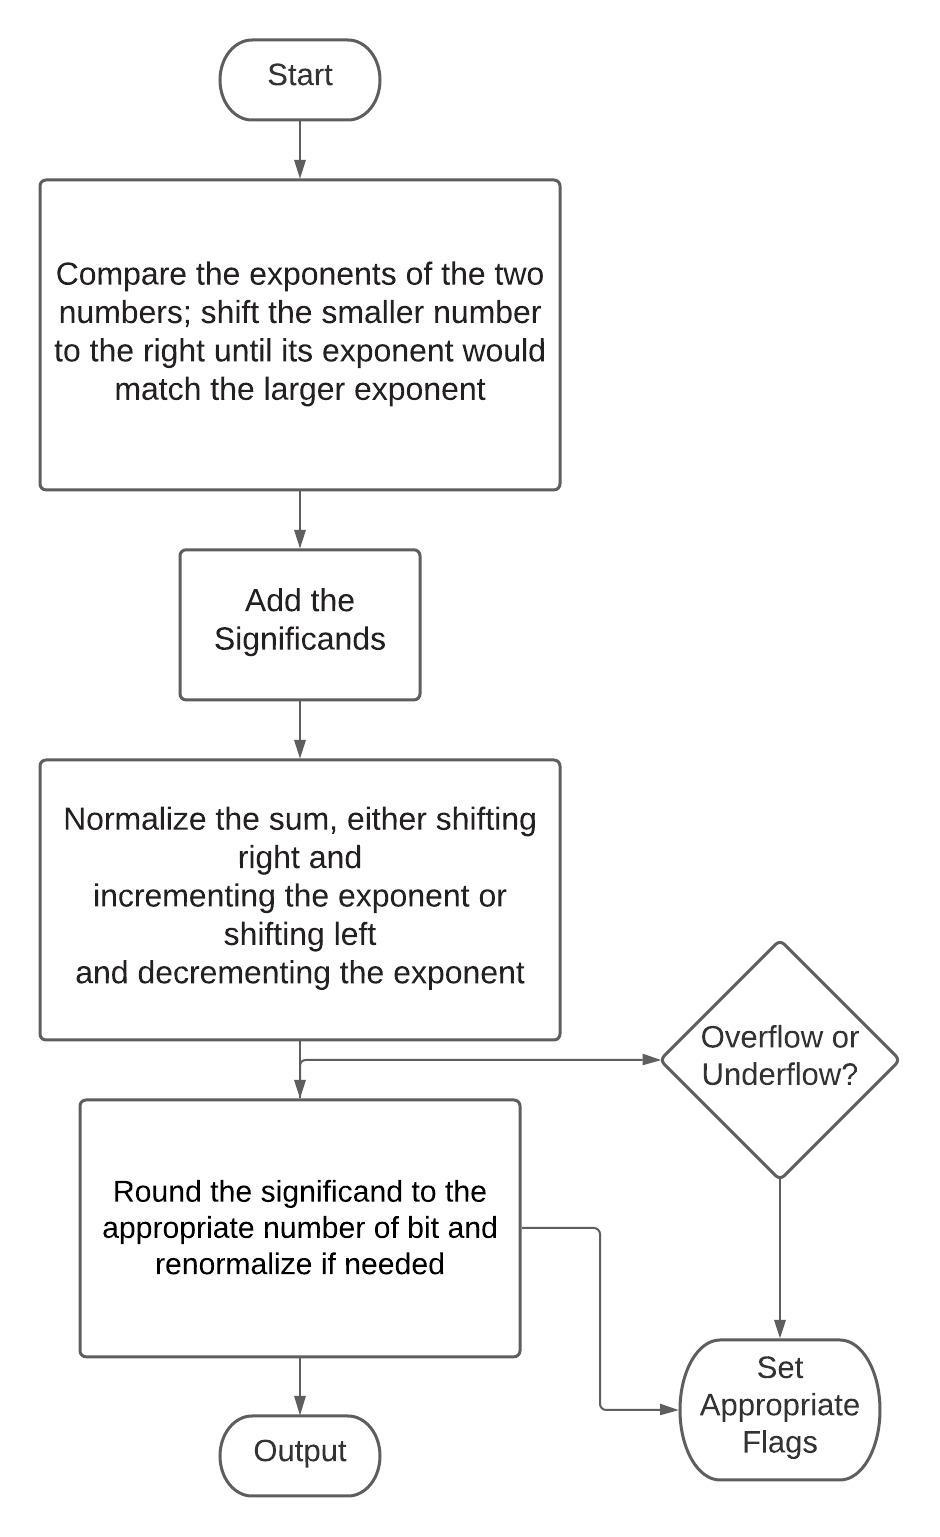
\includegraphics[width = 0.7\linewidth]{algo}
		\caption{Floating Point Addition}
		\label{fig1}
	\end{figure}
	\newpage
	\section{High-Level Block Diagram}
	A very high-level block diagram of the floating point adder is shown in Figure \ref{fig2}
	\begin{figure}[h!]
		\centering
		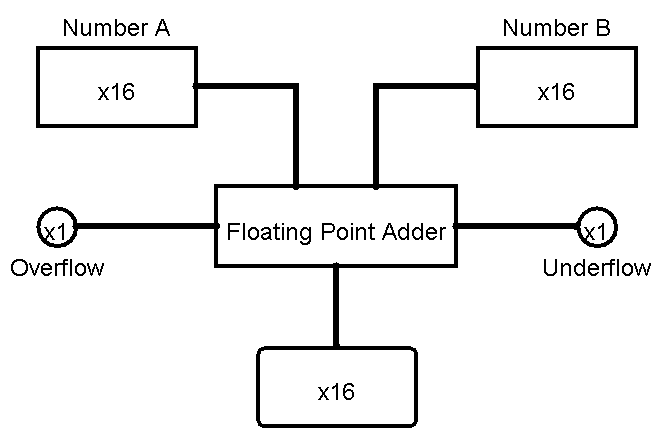
\includegraphics[width = 0.7\linewidth]{block_diagram}
		\caption{High-level Block Diagram of the Floating Point Adder}
		\label{fig2}
	\end{figure}
	\newpage
	\section{FPA Block Diagram}
	The detailed block diagram with all the components is shown in Figure \ref{fig3}
	\begin{figure}[h!]
		\centering
		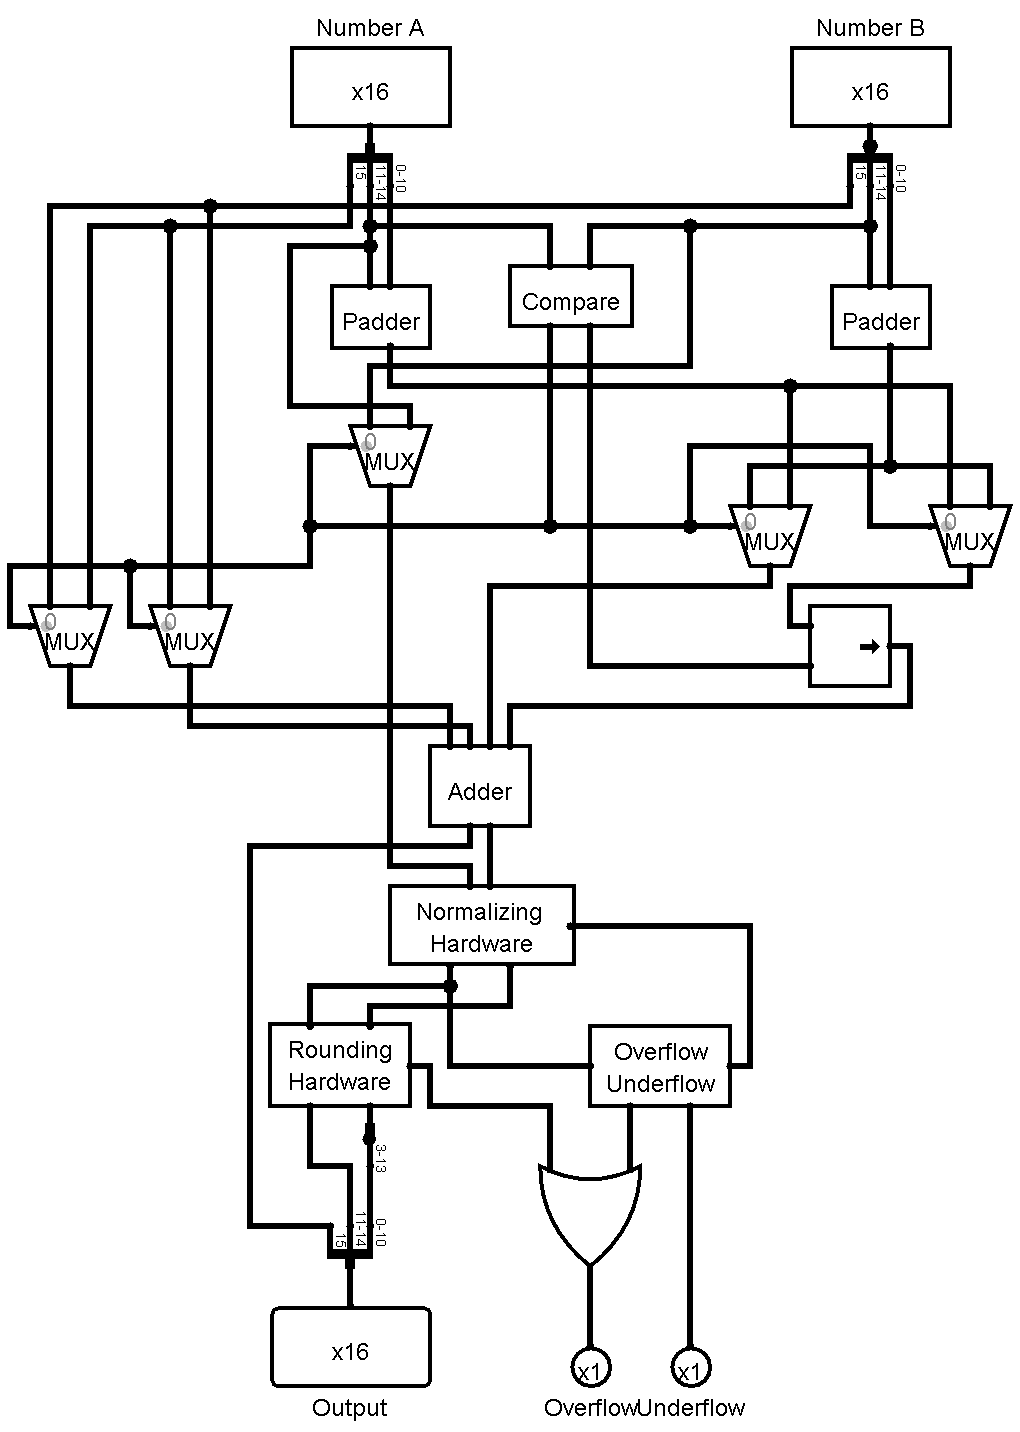
\includegraphics[scale = 0.35]{fpa}
		\caption{Block Diagram of the components inside Floating Point Adder}
		\label{fig3}
	\end{figure}
	\newpage
	\section{Overview of the components}
	\subsection{Compare Block}
	The Compare block compares the exponents and outputs the absolute value of
	their difference. It contains a 4-bit subtractor whose output, $(B-A)$, is
	sent to a MUX both directly and in negated form. The 4-bit negator performs
	2's complement on its input. If $ A > B$, the borrow out is 1 and the MUX
	outputs the negated value of subtractor to get the absolute difference.
	Otherwise, if $B > A$, the direct value is output.
	\begin{figure}[h!]
		\centering
		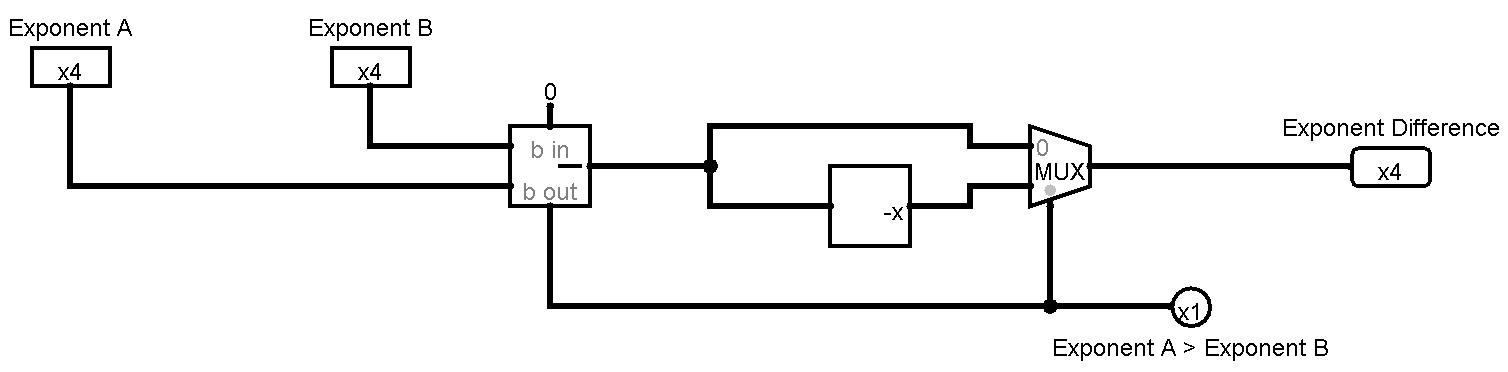
\includegraphics[width = \linewidth]{compare}
		\caption{Circuit Diagram of the Compare Block}
		\label{fig4}
	\end{figure}
	\subsection{Padder}
	The padder converts the 11 bit fraction to a 16 bit significand
	as follows:
	$$Significand = 0X\;\,11\!-\!bitFraction\;\,000$$
	The 0X padded to the left represents two binary digits to the left
	of the binary point. Here X is 1 if the exponent is non-zero, otherwise X
	is 0. These two extra binary bits make the normalization hardware much
	simpler.
	The 000 padded to the right allows us to perform rounding later on. While
	padding with one extra bit to the right would have been enough, we store
	three extra bits because the IC count for both 14-bit and 16-bit adders/MUX
	are same when they are built by cascading 4-bit units. So the two extra bits
	reduce the precision lost during shifting without affecting the IC count.
	\begin{figure}[h!]
		\centering
		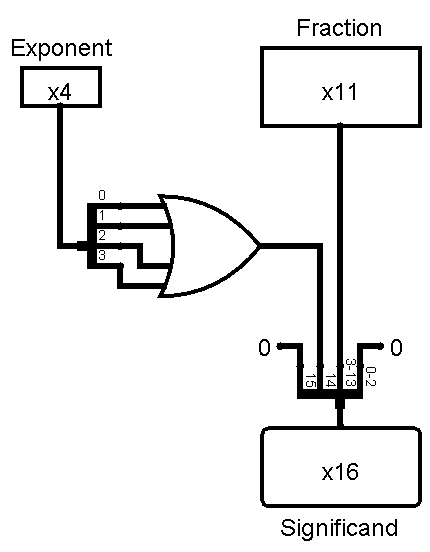
\includegraphics[scale = 0.3]{padder}
		\caption{Circuit Diagram of the Padder Block}
		\label{fig5}
	\end{figure}
	\subsection{Series of MUXs}
	We have a series of MUXs each of which use the ($Exponent A > Exponent B$)
	output from the Compare Block as their selection bit. These MUXs are used
	as follows:
	\begin{itemize}
		\item One MUX to select the larger Exponent
		\item One MUX to select the Significand with the larger Exponent and
		another MUX to select its corresponding Sign
		\item One MUX to select the Significand with the smaller Exponent and
		another
		MUX to select its corresponding Sign
	\end{itemize}
	\begin{figure}[h!]
		\centering
		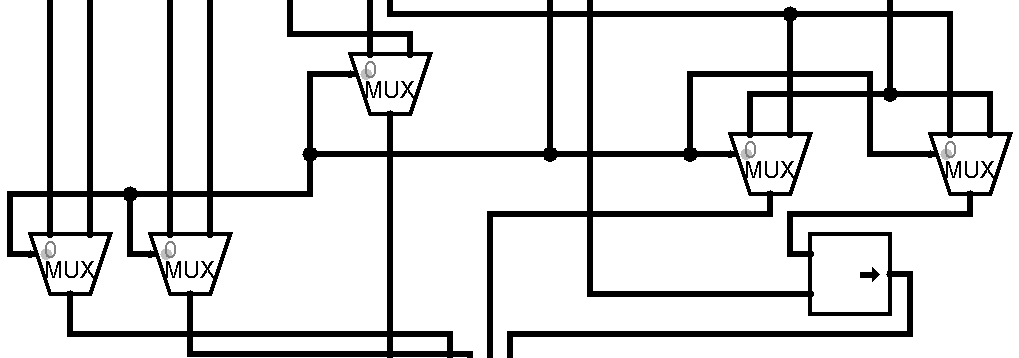
\includegraphics[width = 0.7\linewidth]{mux}
		\caption{Circuit Diagram of the Series of MUXs}
		\label{fig6}
	\end{figure}
	\subsection{Shifter}
	We want the exponent part of both the numbers to be the same before they are
	added. For this purpose the shifter is used which right-shifts the
	significand of the number with the smaller exponent. The shift amount is
	determined by the absolute value of the difference between the exponents.
	We are not providing any diagram showing the internal implementation of the
	shifter because we used the shifter circuit readily provided by Logisim.
	\subsection{Adder}
	The input to the Adder are the two Significands and their corresponding
	Signs.

	The Adder block adds the 16-bit Significants. It contains a Comparator, MUXs, Negator and a 16-bit Adder.

	If $significand1 >= significand2:$ a MUX sends Significand 1 directly to
	the Adder; another MUX sends Significand 2 to a third MUX in both original
	and negated form. This MUX sends the negated form of Significand 2 to the
	adder if the signs are different (XOR of sign bits). Otherwise the original
	form of Significand 2 is sent to the adder.

	If $significand1 < significand2:$ a MUX sends Significand 2 directly to the
	Adder; another MUX sends Significand 1 to a third MUX in both original and
	negated form. This MUX sends the negated form of Significand 1 to the adder
	if the signs are different (XOR of sign bits). Otherwise the original form
	of Significand 1 is sent to the adder.

	Since in both cases the larger value is sent directly to the adder and the smaller one is negated (if signs are different), subtraction produces absolute difference. This is important as we do not need to deal with complements in the answer.

	Finally, we have a MUX for the two signs. The output of the Comparator  is
	used by a MUX to select the sign of the larger Significand as the output
	sign.
	\begin{figure}[h!]
		\centering
		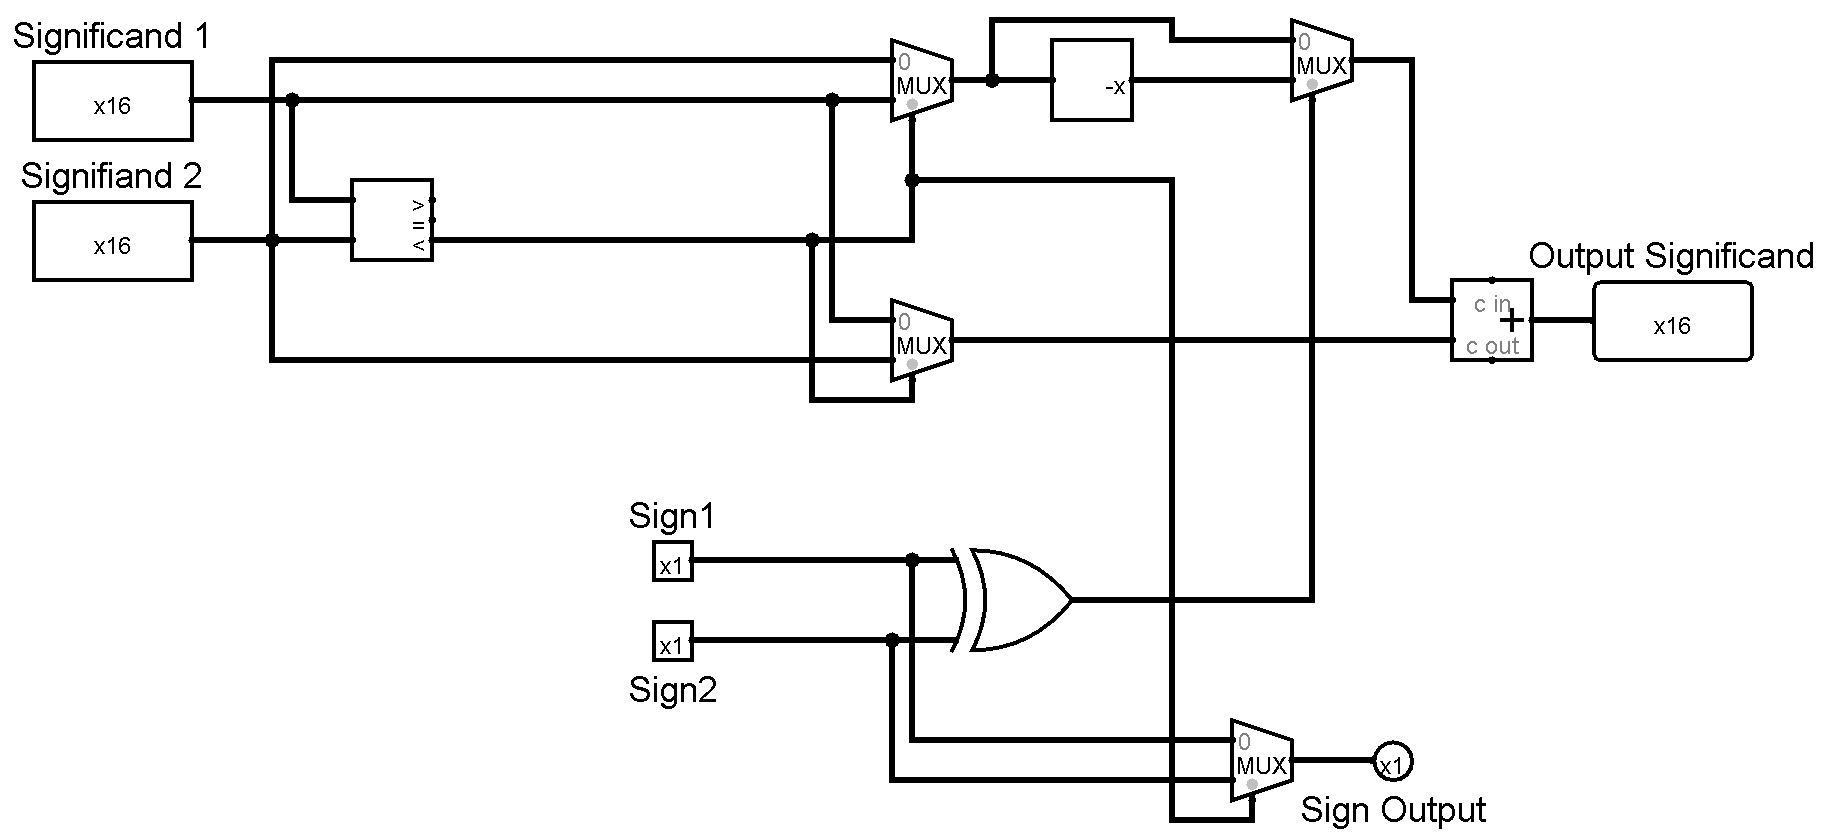
\includegraphics[width = \linewidth]{adder}
		\caption{Circuit Diagram of the Adder Block}
		\label{fig7}
	\end{figure}
	\subsection{Normalizing Hardware}
	In this component the input is a 4-bit Exponent and 16-bit Significand; the output Exponent and Significand are in normalized form
	if normalization is possible. Otherwise the output maybe a Denormal number, or 0, or infinity. Additionally, another output tells
	if the Significand had 0-bits only.
	\newline

	The Normalization Hardware makes use of a Set Bit Finder component which outputs the following:
	\begin{itemize}
		\item If any 1 is present in the Significand
		\item The number of positions the highest set bit needs to be shifted for the output to be in normalized form.
	\end{itemize}

	For Normalization left shift by 0-14 bits might be needed, or right shift by 1 bit maybe needed. To simplify the situation we used
	Left Rotator instead because left rotation by 15 bits is the same as right shift by 1 bit in this case.

	If the amount of left shift needed is greater than or equal to the value of the exponent, then the output will be a Denormal number.
	The Significand is shifted Exponent-1 times to the left and the output Exponent is 0000.

	If the value of the output Exponent is 1111, then it is a case of overflow. And according to IEEE-754's representation of infinity, the Fraction part of the Significand is made all 0s.
	\begin{figure}[h!]
		\centering
		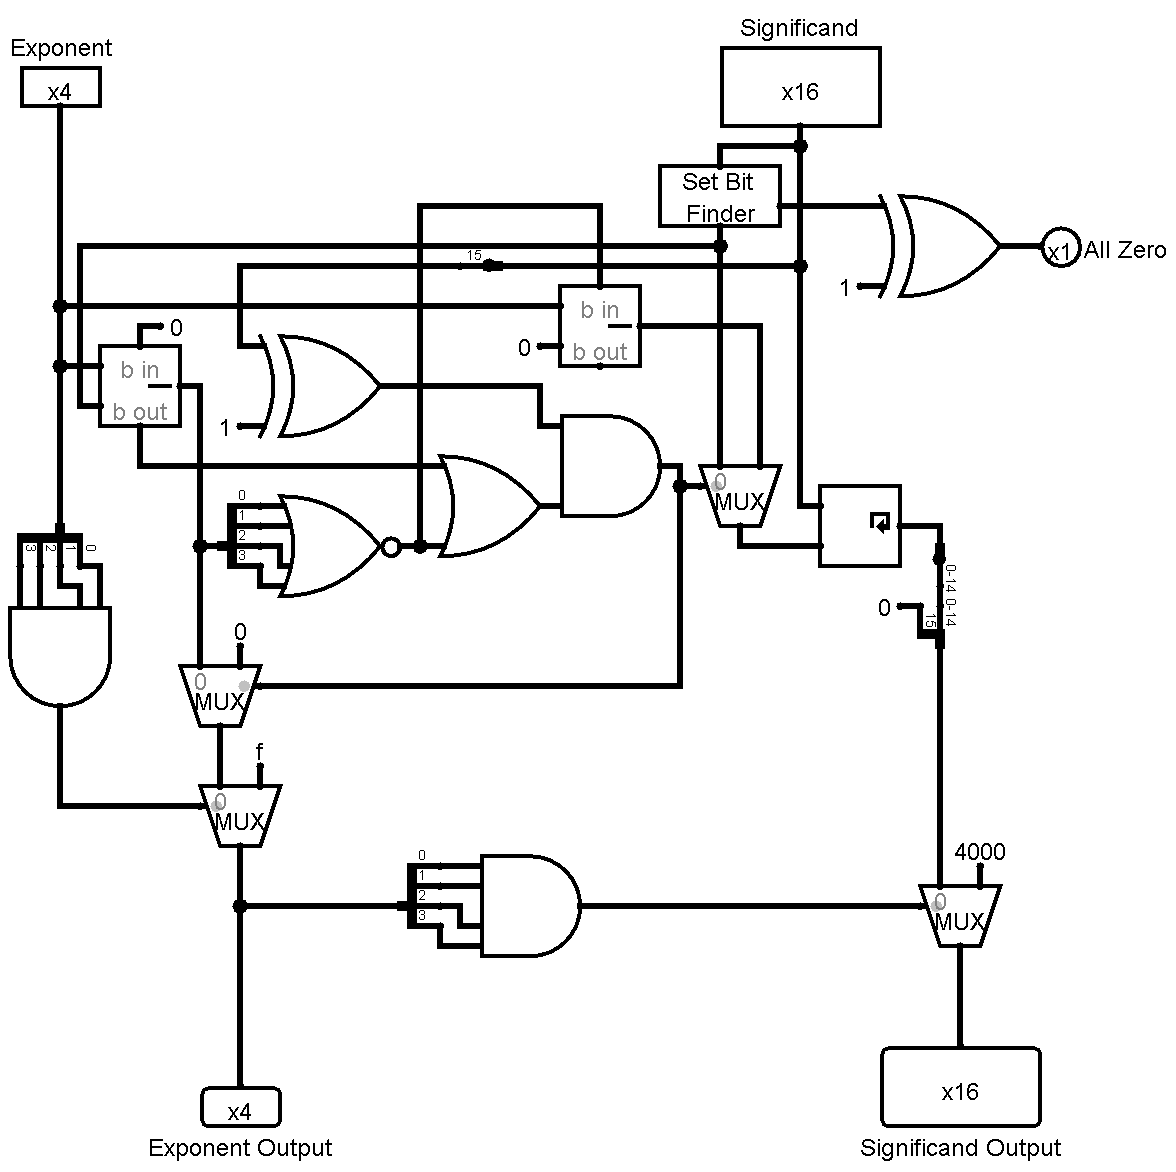
\includegraphics[width = 0.7\linewidth]{nhw}
		\caption{Circuit Diagram of the Normalization Hardware}
		\label{fig8}
	\end{figure}
	\subsection{Set Bit Finder}
	It takes the 16-bit Significand as input and then reverses the input. The index of the lowest set bit is found and 1 is subtracted from it. The resulting value is equal to the number of left rotation needed for the Significand to be converted to Normalized form.
	\begin{figure}[h!]
		\centering
		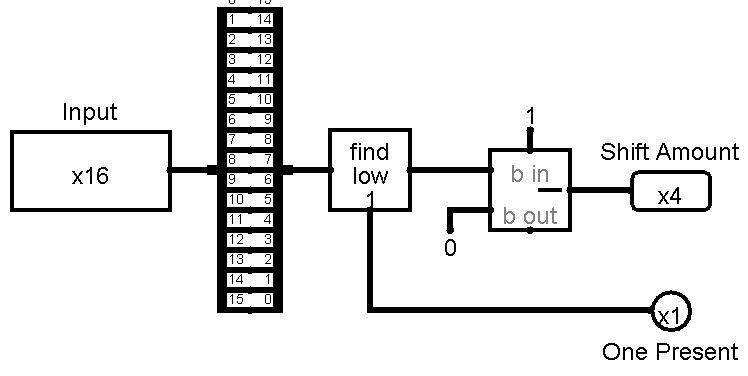
\includegraphics[width = 0.8\linewidth]{setbit}
		\caption{Circuit Diagram of the Set Bit Finder}
		\label{fig9}
	\end{figure}
	\subsection{Rounding Hardware}
	We have taken the Significand and Exponent as input and given as output the
	the final Significand, Exponent and Overflow detection. We check the 3rd
	bit from right to understand if rounding is needed.
	If the 3rd bit from right is 1, we round the Significand by adding it to a
	binary number with 1 at the 4th bit from right and 0's elsewhere.
	If rounding causes number to become un-normalized, we right shift the
	Significand by 1 and add 1 to the Exponent.
	\begin{figure}[h!]
		\centering
		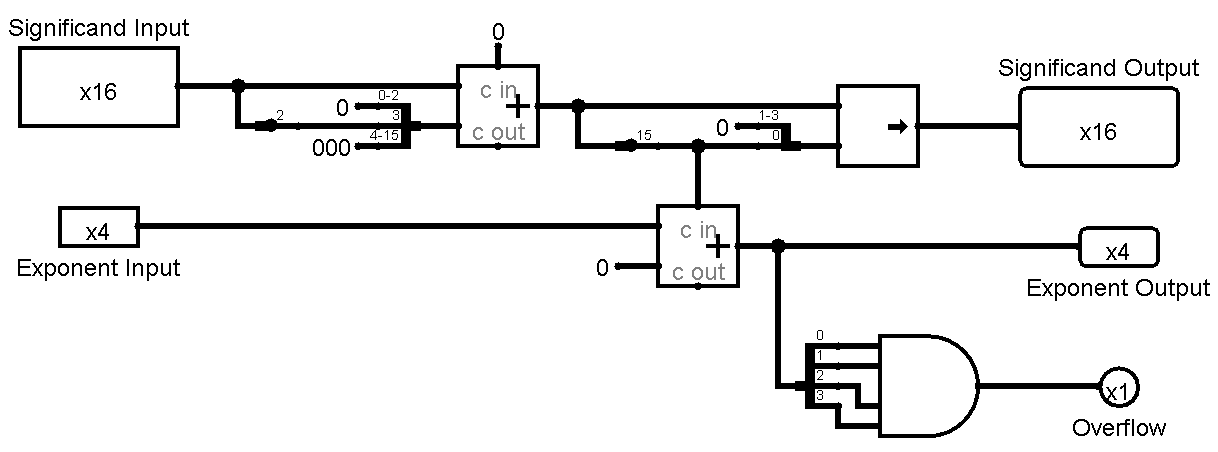
\includegraphics[scale = 0.35]{round}
		\caption{Circuit Diagram of the Rounding Hardware}
		\label{fig10}
	\end{figure}
	\subsection{Overflow/Underflow}
	Overflow occurs when all bits of the Exponent are 1. Underflow occurs
	when all bits of the Exponent are 0 but all bits of the Significand are
	not 0
	\begin{figure}[h!]
		\centering
		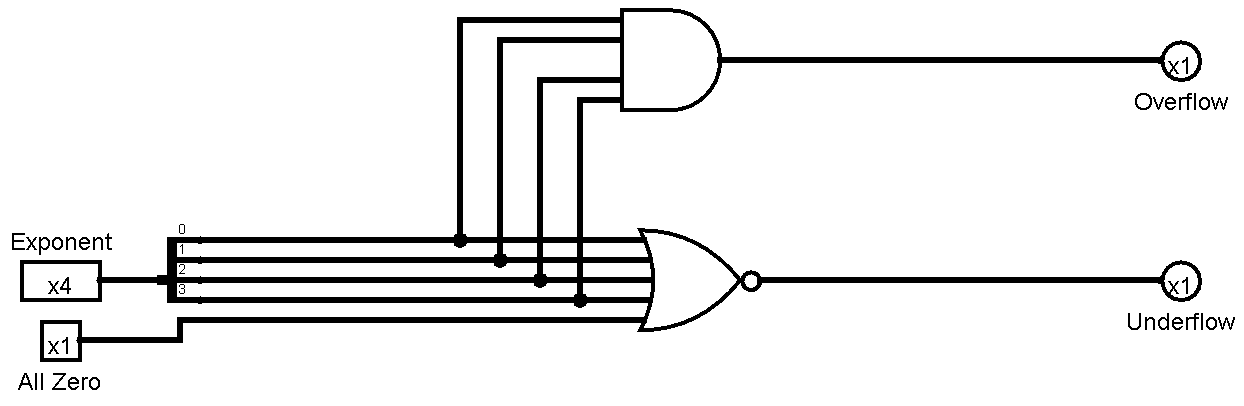
\includegraphics[width = 0.9\linewidth]{over}
		\caption{Circuit Diagram of the Overflow/Underflow detector}
		\label{fig11}
	\end{figure}

	\section{IC Count}
	\begin{table}[H]
	\centering
\begin{tabular}{|l|l|l|l|} \hline
Operation        & Total & IC     & No Of Ics  \\ \hline
QUAD 2-AND       & 1     & 7408   & 1          \\ \hline
DUAL 4-AND       & 4     & 7421   & 2          \\ \hline
QUAD 2-OR        & 2     & 7432   & 1          \\ \hline
DUAL 4-OR        & 1     & 744072 & 1          \\ \hline
QUAD 2-XOR       & 7     & 7486   & 2          \\ \hline
DUAL 4-NOR       & 2     & 7429   & 1          \\ \hline
4 bit Adder      & 9     & 7483   & 9          \\ \hline
4 bit Comparator & 4     & 7485   & 4          \\ \hline
16 bit Shifter   & 3     & -      &            \\ \hline
4 bit Subtractor & 4     & -      &            \\ \hline
Bit Finder       & 1     & -      &            \\ \hline
4 bit Negator    & 5     & -      &            \\ \hline
Quad 2:1 MUX     & 119   & 74157  & 30         \\ \hline
                 &       &        & Total : 51 \\ \hline
\end{tabular}
\end{table}

	\section{Simulation Platform}
	Logisim-2.7.10
	\section{Discussion}
		About a week before the submission deadline the problem was simplified
		as follows:
		\begin{itemize}
			\item The input numbers would strictly be in Normalized form
			\item Truncation was allowed instead of rounding
		\end{itemize}
		However by that time we had already progressed significantly with our
		work where we had handled inputs in Normalized/Denormal/0/Infinity
		form. Also we had implemented rounding instead of truncation as per the
		original specification. So we believe the large number ICs required in
		our implementation is due to the additional functionality - not due to
		any form of inefficiency in circuit design.
		\newline

		We assumed that IC minimization across different components is allowed.
		For example: 2 XOR gates were required in the Normalization Hardware
		and 1 XOR gate was required in the Adder. We assumed all three of these
		can be implemented using the same 7486-XOR gate.
		\newline

		After rounding the number can become un-normalized. So it must be fed
		back to the Normalization Hardware. However, this means the process
		would involve clock pulses. To avoid the use of clock pulses we
		identified the specific scenario where this problem would occur and
		handled it separately. This means our circuit remains a combinational
		one, however this approach does increase IC count slightly.

\end{document}
